\section{Modules Selection}

The previous chapter explains the libraries used in this testbed and discloses some of the components that construct the testing environment. This chapter points out the significance of picking certain hardwares and modules other than the software support. Mainly, when considering parts for the testbed, the project focuses on the hardware capability and cost. 

In terms of functionality, a CR device must be able to sense the environment and react to the current situation. Since it needs to sense the spectrum in the air, it requires some sort of receiver with an antenna. To be able to also send data in the air, it requires a transmitter. CC1101 module composes a CC1101 transceiver chip, a SubMiniature version A (SMA) antenna, and circuitry that wires between the chip and the interface. A 3D model of the hardware module is shown in Figure~\ref{fig:cc1101_module}. 

\begin{figure}[ht]
\centering
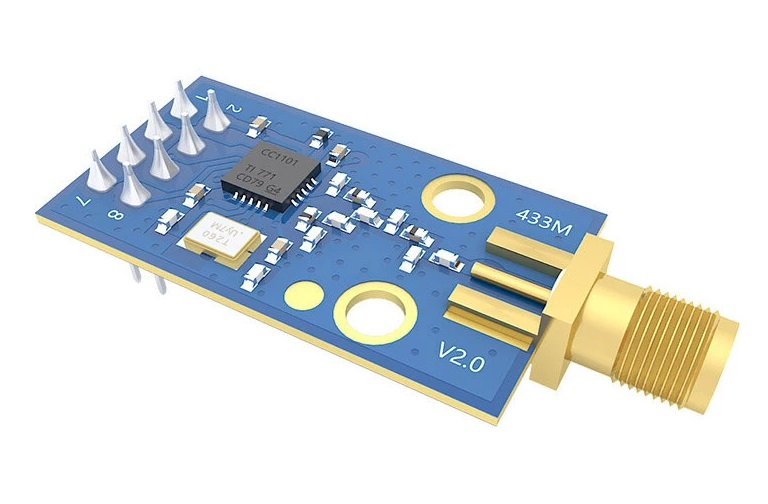
\includegraphics[width=14cm]{figures/cc1101_module.jpg}
\caption{CC1101 Transceiver Module}
\label{fig:cc1101_module}
\end{figure}

The hardware characteristics of CC1101 module are qualified in the following areas. All input required a voltage level below 3.6 V \cite{cc1101_module}. The operating current is well under 30 mA. If the typical operating I/O voltage is 3.3 V, the peak power is under 100 mW, which is acceptable for a testbed usage. It can transmit at a frequency range of 387 - 464 Mhz; the range falls in VHF range, which will fulfill the purpose of this project. The operation range of the transceiver can reach about 520 meters. It is capable of communicating with MCU through SPI. The operating temperature is designed for room temperature; it specified to be between 40 - 85 \textdegree{}C.

CC1101 module would only produce the environmental data that the CR device needs. There should be another module that processes the generated digital data from the transceiver. There are many hardwares that can process digital data, such as the single-chip microcontroller, field-programmable gate array(FPGA), digital signal processor (DSP), etc. Above all these, a well developed module board comes to mind; the Arduino Nano is the best candidate for this project due to its strong hardware support and flexible compatibility. The 3D model of this module is shown in Figure~\ref{fig:arduino_nano}. 

\begin{figure}[ht]
\centering
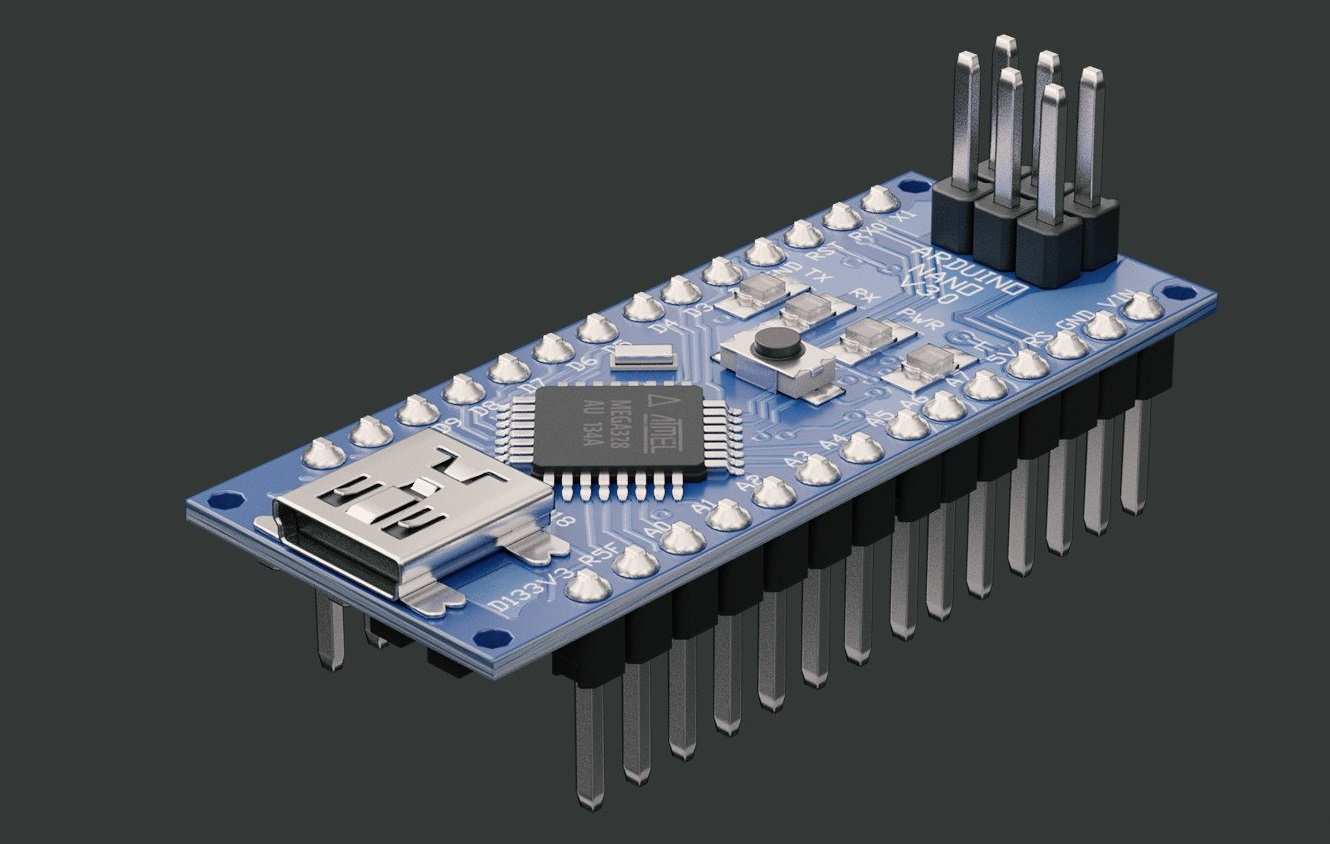
\includegraphics[width=12cm]{figures/arduino_nano.jpg}
\caption{Arduino Nano Module}
\label{fig:arduino_nano}
\end{figure}

Arduino Nano uses the ATMEGA328 chip for the core of the part. Inside ATMEG328 there is a micro process unit that can run in various clock speed by dividing the default clock, 16 Mhz. In addition, ATMEGA328 has a built in EEPROM with 1 kB capacity for data storage. That fulfill the project's data recording need. Since it is used to drive the the rest of the peripherals, it needs to produce a powerful I/O driven current. The data sheet shows it is capable of providing 40 mA per I/O pins. A 5 V operating voltage is perfect for the level shifters that have been selected for the project. The input voltage has a range from 7 - 12 V; this provides ranges of voltage-level for a 9 V running battery. There are plenty of digital I/O pins for all the traveling signal across the components. Its tiny size and power hardware make it stand out from the rest of MCU.


Furthermore, the testbed needs a control for starting the test. It is as simple as adding a switch that connects to the power. Lastly, during the experiment, the user should find it beneficial to have some kinds of indication of the device's performance or status. By flashing the LEDs at certain stages of the experiment process, the user can estimate the testing progress on the run. Figure~\ref{fig:block_diagram} shows the full top-level diagram. Note that in the final design, there are two sets of level-shifters between MCU and the transceiver module because the Arduino Nano produces and receives 5 V I/O, where as CC1101 generates and takes in 3.3 V I/O. The components are generally easier to get with low prices. For the complete data sheet of all the hardware modules, please refer to Table X, Table Y, Table Z in the Appendix. For the full Bill of Material, please refer to Table~\ref{tab:bill} in the Appendix as well.

\begin{figure}[ht]
\centering
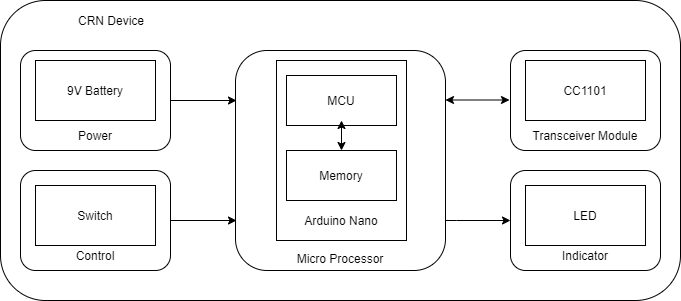
\includegraphics[width=12cm]{figures/new_block_diagram.png}
\caption{Top Level Block Diagram}
\label{fig:block_diagram}
\end{figure}


\section{Prototype Board}

The CRN testbed includes three different types of devices, BS, CPEs and LBUs. However, for the board development, all three types of devices are actually made by the same hardware layout. By uploading unique software programs, they behave differently. Figure~\ref{fig:prototype_board} is the complete prototype board schematic of the device. The figure is a back panel of the device with the exact wire routing to each nodes.

\begin{figure}[ht]
\centering
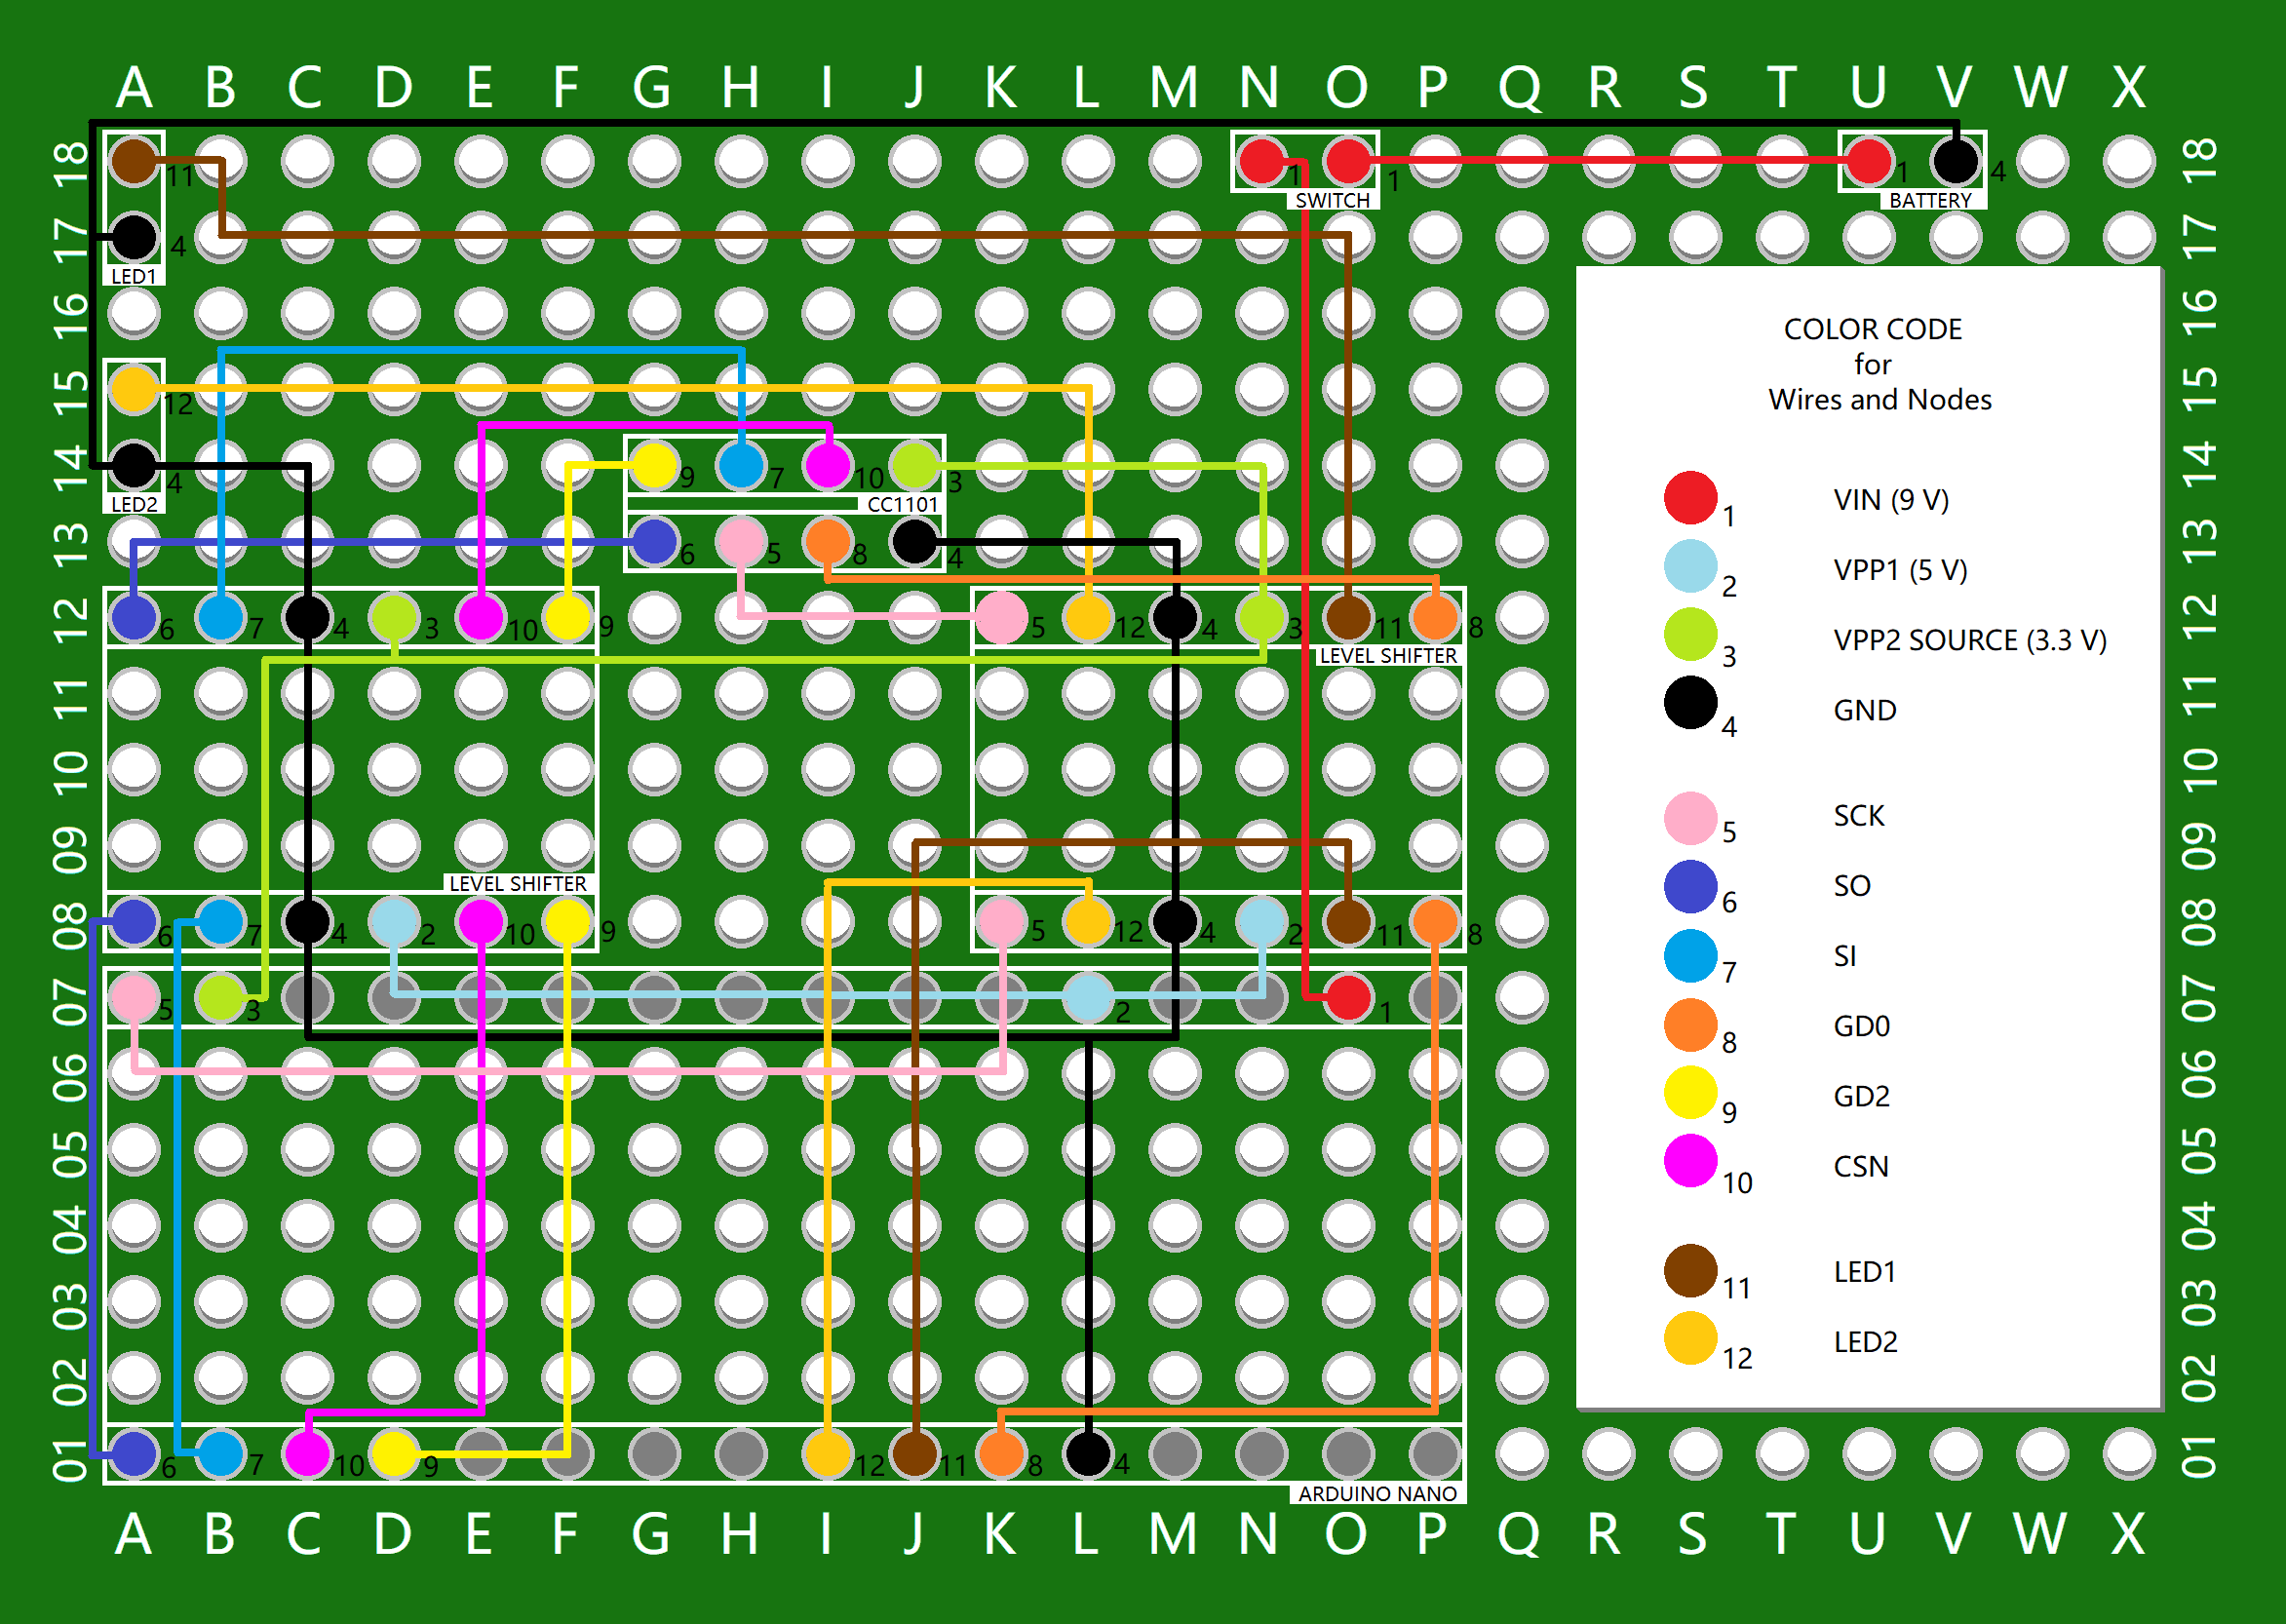
\includegraphics[width=14cm]{figures/clean_prototype_board.png}
\caption{Prototype Board Pin out and Wire}
\label{fig:prototype_board}
\end{figure}

After optimizing the placement and the wiring, components can fit on a 5x7 centimeter prototype board. On the side, there are reserved spaces for the power, and just enough space for a 9 V battery. The power switch, located at the top center of the board, is connected to the Arduino Nano power input and the power connector of the battery. The two LED indicators are located on the far top corner. One is blue; the other one is yellow. Toward the middle are a pair of soldered headers for the transceiver module. The two signal level-shifters are placed in the center of the layout. Each level shifter module is capable of shifting four I/Os. Two level-shifters are enough for all necessary signals in this project. On the bottom is the Aruidno Nano. The power drives the Aruidno machine; the Aruidno drives all the rest of the peripherals. Each color coded line represents a same wire connecting the pins and the headers. The legend on the side shows the color and number of the node and its corresponding pin name. With the detailed layout, the components are assembled into hand soldered devices, referring to Figure X and Figure X for a prototype at the Appendix.

One challenge putting together the components on the prototype board is the hand soldering part. All the components can be found on the front side of the board panel, while the wiring is hiding at the back panel. Each slot that needs to be soldered - most of these slots are big nodes - have two or three wires going into them. With the header pin that plugs from the front through the back, it may be  difficult for the single node to accommodate all wires during the soldering process. To avoid shorting at the crossing wire, the wires are conductive material with plastic insulator around it. The metal only exposes about 5mm towards both ends. The headers are placed at the designated prototype pin holes. Taking the height of the components into consideration, the orientation of the headers must be accurate and straight in order to fit in this limited space. Inserting headers are extremely beneficial for this project in the long run. The board, headers, and wires arrange the interconnection of the device. Components such as Arduino Nano, levels shifters, battery, and transceiver can be plugged in to use. While certain hardware parts may fail, users can replace those hardware components without dissembling the whole board. When upgrading the prototype, all the components can be recycled and used for the next project. This method helps the devices' sustainability. For the Bill of Material of the full board, please refer to Table~\ref{tab:bill} in the Appendix.


\section{Verification}

This hardware design passes a series of functional unit-tests and fulfills all requirements for a CR testbed. Below are the physical confirmation of the component use cases and the test methods.

\begin{itemize}
  \item components I/O current conforms the specification\newline
  Method: Arduino Nano data sheet shows that 40 mA of current can be generated to drive other load. 40 mA of driven current is well above requirement of both the level-shifters and transceiver, which is shown in their data sheet.
  \item transmission stays stable within range\newline
  Method: They are tested with constant transmission and receiving functionality within ten minutes of operation duration and ten meter of ranges in room temperature.
  \item batteries are capable for running number of experiment runs.\newline
  Method: A 9 V battery is advsertised to have 500 mAh charge capacity. It is capable for a single device to run five or more hours.
\end{itemize}

Below are the list of behavioral confirmations of the system.

\begin{itemize}
  \item BS recognizes and identifies all types of devices\newline
  Method: Within the synchronization phase, the BS can receive the message from all devices with specific protocol and insert them into the ready-list. LED indicators from the BS flashes to confirm this process.
  \item LBU and CPE connect to BS \newline
  Method: LBU and CPE connect to the BS separately. LED indicators from LBU and the CPE flashes to confirm this process.
  \item LBU and CPE synchronize with BS\newline
  Method: After synchronization process, all LED indicators flash at the same time as they begin the experiment.
  \item LBU reads its unique schedule from the \texttt{TEST} library and switches channels\newline
  Method: LBU transmits in designated channels at certain time periods that are specified in the \texttt{TEST} library.
  \item CPE recognizes the termination time\newline
  Method: CPE reads and compares current time and termination time defined in the \texttt{TEST} library. When they match, it will end the experiment.
  \item CPE records data to and output data from the \texttt{EEPROM}\newline
  Method: CPE can write to the \texttt{EEPROM} and read from the \texttt{EEPROM}. It is confirmed by a simple read and write program.
  \item CPE would delay prime number amount of time when receiving no response during requesting state\newline
  Method: During the requesting state, after the CPE sends out the message and timer expires, CPE will wait for the series list of prime number time delay to begin the next attempt.
  \item CPE senses if the channel is free or busy\newline
  Method: CPE immediately hops out of the assigned channel if LBU is already transmitting. During CPE transmission, it will hop back to reserve channel if the LBU happens to intercept in the middle.
  \item BS detects LBU\newline
  Method: In the periodic sensing function, BS can detect the environment with the confirmation of the LED indicators.
  \item BS selects a valid channel\newline 
  Method: Experiment with LBUs occupying the specific channel cause BS to choose the specific one. 
  \item BS updates channel and client status\newline
  Method: BS prints out all the channel and client statuses at some simple test cases. It updates the status lists whenever there is a change.
  \item BS updates selection table\newline
  Method: BS prints out selection at some simple test cases. It updates the selection table and makes the best decision.
\end{itemize}
